\subsection{Planejamento de trajetória}

\subsubsection{Modelagem da superfície}\label{modelagem}

%
%Book
%Geometry and Computing
%Volume 3 2008
%Subdivision Surfaces
%Authors: Jörg Peters, Ulrich Reif
%ISBN: 978-3-540-76405-2 (Print) 978-3-540-76406-9 (Online)

% BEZIER
%Farin, Gerald. Curves and Surfaces for CAGD (5th ed.). Academic Press. ISBN
% 1-55860-737-4.




Existem diversas abordagens matemáticas para descrição de superfícies como:
Parametrização Polinomial; Polinômios em três variáveis; Superfícies de
Bézier; Splines e NURBS (\textit{Non-uniform rational B-spline}); Subdivisão de
superfícies; Malhas poligonais.

Todas essas formas de representar uma superfície, com excessão das malhas,
recaem em alguma instância em uma descrição polinomial. Dentre essas o única
descrição que ocorre de maneira implícita é por polinômios em três variáveis,
descrevendo uma variedade algébrica bidimensional, enquanto as demais são
parametrizações da superfície. 

Por simplicidade, fácil manipulação algébria e implementação, a descrição
puramente polinomial (implícita) foi escolhida como abordagem inicial. De
maneira geral a superfície é descrita como o conjunto solução sobre os
reais da equação polinomial ($f(x,y,z)=0$) de grau $N$, dito grau da
superfície, em $x$,$y$ e $z$:
\[\sum\limits_{i+j+k \leq N}^{} C_{i,j,k}x^iy^jz^k = 0\]

Os coeficientes $C_{i,j,k}$, então, são aqueles que descrevem da superfície.
Devido a restrição do grau do polinômio, o número de coeficientes é
$\binom{N+3}{3}$.

Experimentalmente foi indentificado que um polinômio de quarto grau é suficiente
para aproximar toda uma região de interesse da pá, onde será feito o coating
para uma posição do robô, com erro submilimétrico. Nesse caso, o número de
coeficientes que devem ser identificados é $\binom{7}{3}$, ou seja, 35.

% TODO nome do artigo
Com base no artigo !!!!!!! a passagem da descrição da superfície por nuvem de
pontos para analítica foi feita utilizando a informação da direção da normal à
superfície em cada ponto. Para isso o peso dado a importância da superfície
descrita concordar com a normal em cada ponto foi o mesmo que o peso dado para
que a superfície passe por esse ponto.

Explorando o fato que polinômio são lineares em seus coeficientes, um sistema
superdeterminado, a ser resolvido por mínimo quadrados, foi contruído a partir
do cálculo dos termos do polinômio em cada ponto da nuvem (fazendo $f(x,y,z)=0$)
e da avaliação da normal em cada ponto, que deveria concordar com o gradiente do
polinômio (ou seja $\nabla f(x,y,z) = \overrightarrow{n}$, onde $\overrightarrow{n}$ é a normal no ponto $(x,y,z)$ da nuvem).

%Elael Modelo Polinomial multivarial -> extrapolado para a pá inteira
% PREMISSAS!!


% 
% Splines
% Bézier Surface
% Runge's phenomenon
% Multivariate Polynomial fitting


\subsubsection{Cálculo dos paralelos}
% como subdividir em segmentos as regiões PREMISSAS!!
Na literatura, há diversas formas de dividir a superfície a ser revestida em
subregiões. Em \cite{from2010off}, por exemplo, um manipulador realiza a pintura
de uma superfície (\textit{spray gun}) cobrindo subregiões de um plano, projeção
da superfície (figura~\ref{fig::pal}). Outra possibilidade é, em funções
paramétricas, realizar uma trajetória semelhante a~\ref{fig::pal} no espaço dos
parâmetricos, cuja transformação (jacobiano) mapeará nos 'cortes' curvos da
superfície.

\begin{figure}[!ht]
	\centering	
	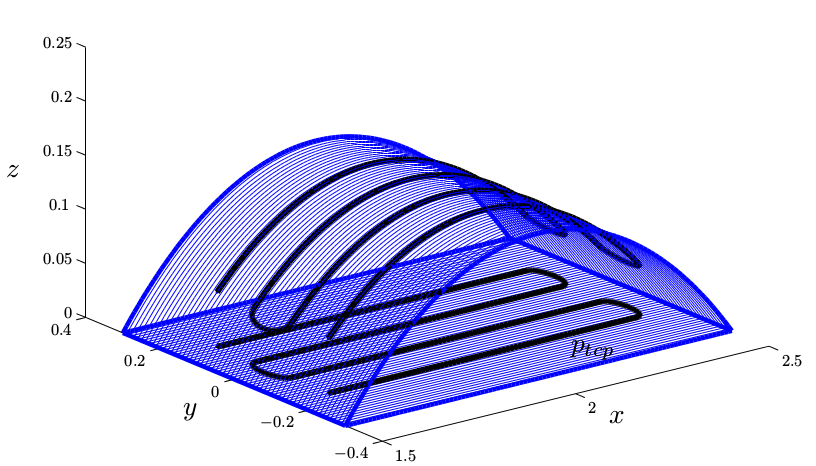
\includegraphics[width=\columnwidth]{figs/planejamento/pal.png}
	\caption{Subregiões de uma superfície.}
	\label{fig::pal}
\end{figure}


A superfície descrita na seção~\ref{modelagem} é uma equação implícita, na forma
$f(x,y,z)=0$. Neste caso, as trajetórias a serem percorridas pelo manipulador
podem ser obtidas através da interseção (cortes) entre planos uniformemente
espaçados e a superfície, o que gerará curvas ao longo da superfície. Uma ideia
semelhante e propícia devido à geometria do rotor, é gerar as curvas a partir da interseção
entre esferas e a superfície. As figuras~\ref{fig::interfrontal}
e~\ref{fig::interiso} mostram duas visões de duas interseções entre esferas e
a pá, onde as interseções estão representadas em vermelho.. Os mesmos cortes
podem ser observados entre esferas e o modelo algébrico da pá, em figura~\ref{fig::intergeo}.


\begin{figure}[t!]
	\centering
	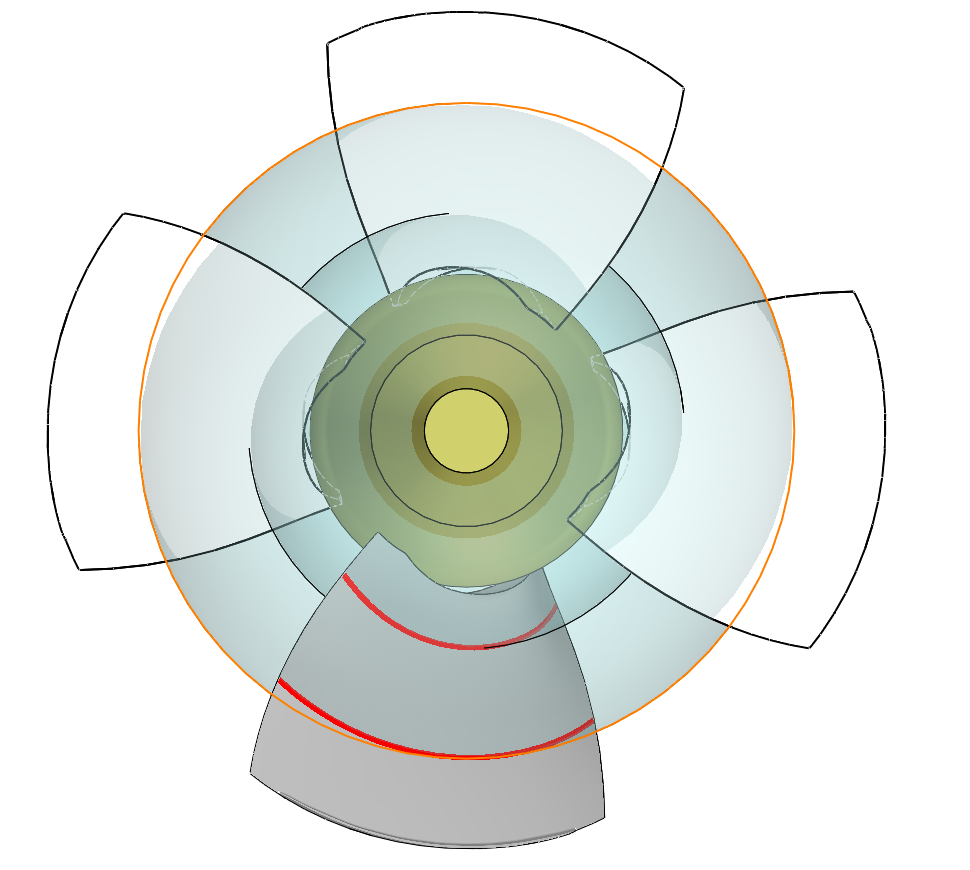
\includegraphics[width=\columnwidth]{figs/planejamento/intersecao_frontal.PNG}
	\caption{Interseção esfera-pá, vista frontal.}
	\label{fig::interfrontal}
\end{figure}

\begin{figure}[t!]
	\centering
	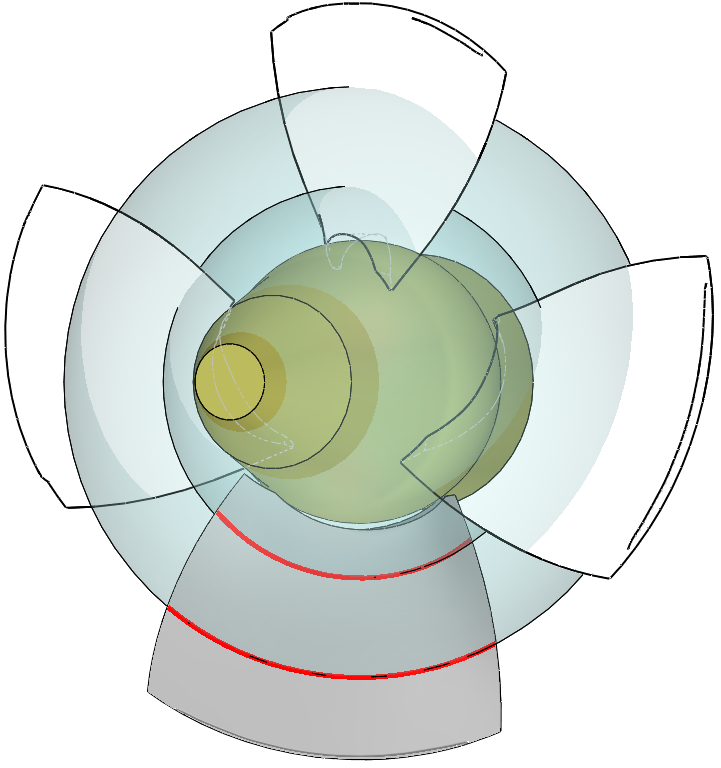
\includegraphics[width=\columnwidth]{figs/planejamento/intersecao_iso.PNG}
	\caption{Interseção esfera-pá, vista isométrica.}
	\label{fig::interiso}
\end{figure}

\begin{figure}[t!]
	\centering
	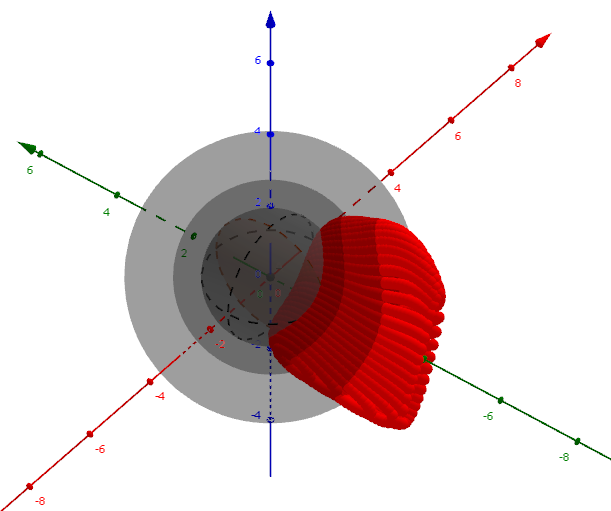
\includegraphics[width=\columnwidth]{figs/planejamento/intersecao_geogebra.png}
	\caption{Interseção esfera-modelo pá.}
	\label{fig::intergeo}
\end{figure}
\subsubsection{Cálculo dos meridianos}
Os paralelos, ou caminhos ``horizontais'', são computados pelo algoritmo
descrito na subseção~\ref{paralelos}. Entretanto, o algoritmo não descreve as
transições entre linhas horizontais, como se o manipulador ``pulasse''
de um paralelo a outro, o que não pode acontecer, já que o caminho deve ser
contínuo. Dessa forma, há a necessidade de computação das curvas de transição,
os caminhos ``verticais'', ou meridianos da superfície da pá.

Ao fim da execução do cálculo de um paralelo (por exemplo, ao fim do
cálculo da curva em vermelho da figura~\ref{fig::interiso}), o
efetuador estará apontando para o último ponto com solução viável neste
paralelo, dentro das restrições de ângulo de revestimento, no lado esquerdo ou direito. A partir
deste ponto extremo (borda), o manipulador deverá ``descer'' ou ``subir'' pelo
meridiano, até encontrar outro paralelo, isto é, encontrar outra curva que
satisfaça $f(x,y,z)=g(x,y,z)$.

O método será explicado a partir de um exemplo genérico: suponha que o efetuador
do manipulador se encontra como na figura~\ref{fig::path_openrave} (borda
direita), isto é, na extremidade direita de um paralelo $c_1$. Caminhar em um
meridiano significa integrar o vetor tangente perpendicular ao encontrado por $\vec{BD} = \vec{OB} \times
\nabla{f}$, logo o caminho pelo meridiano pode ser calculado
como:
$$m_{12} = \int (\vec{OB} \times \nabla{f})\times \nabla{f} dt$$
o que irá gerar um caminho de descida pelo meridiano. Em cada passo de
integração numérica, o novo ponto $B' = B + \int_0^t (\vec{OB} \times
\nabla{f})\times \nabla{f} dt$ deve ser projetado na superfície, como em
na subseção~\ref{paralelos}, pela otimização:
$$min \left \| B-B' \right \|^2$$
$$s.t. f(B')=0$$
Além disso, em cada passo deverá ser verificado se o caminho já alcançou o
próximo paralelo $c_2$, isto é, se o ponto pertence à esfera de raio
$R_2=R_1+0.003$ (em milímetros). Observe que se o o caminho passar do próximo
paralelo, o caminho deve ser feito no sentido contrário com passo menor, isto é:
$$m_{21} = \int -(\vec{OB} \times \nabla{f})\times \nabla{f} dt$$

Na figura~\ref{fig::meridianos}, os meridianos estão representados em verde.

\begin{figure}[!ht]
	\centering
	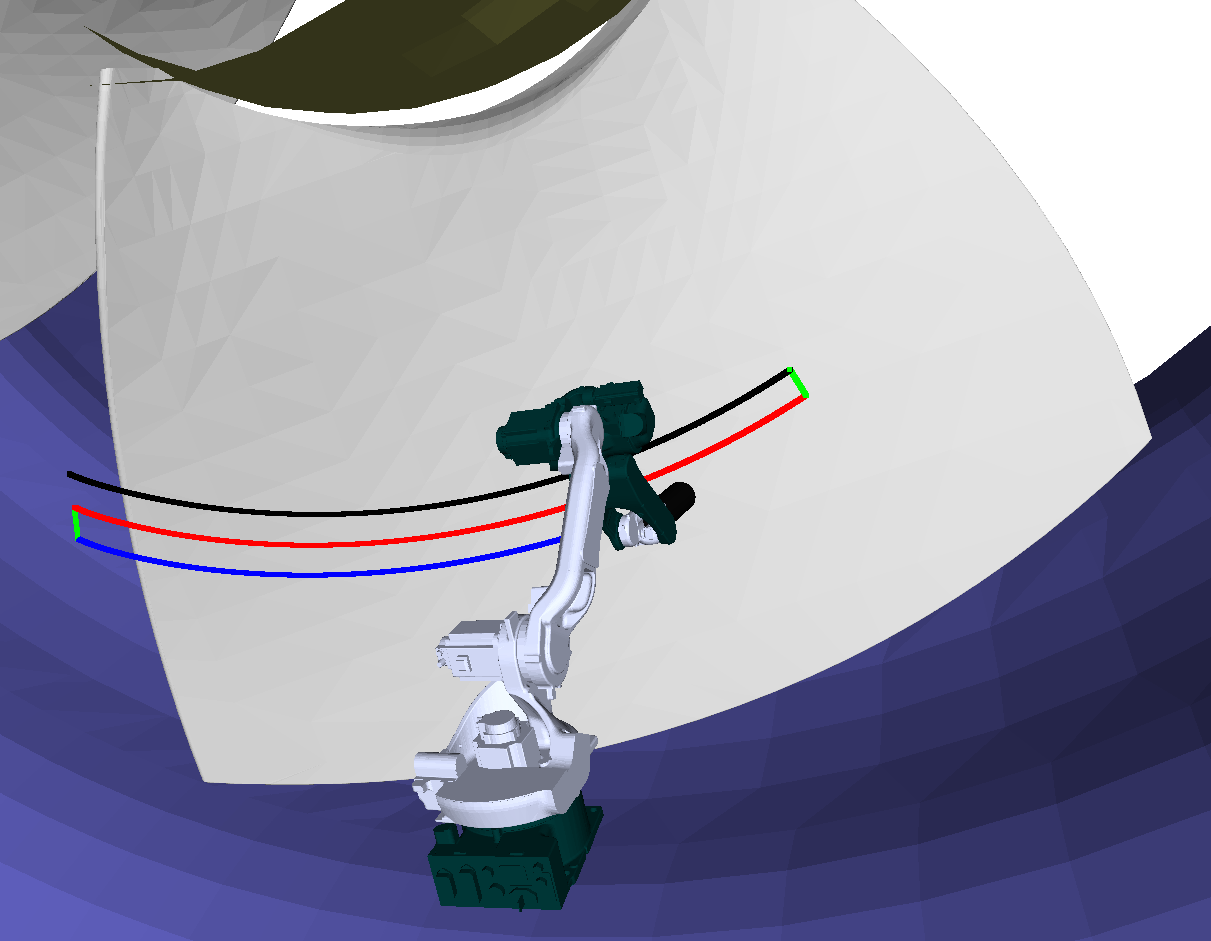
\includegraphics[width=\columnwidth]{figs/planejamento/meridianos.png}
	\caption{Meridianos da pá.}
	\label{fig::meridianos}
\end{figure}